% Template for PLoS
% Version 1.0 January 2009
%
% To compile to pdf, run:
% latex plos.template
% bibtex plos.template
% latex plos.template
% latex plos.template
% dvipdf plos.template

\documentclass[10pt]{article}

% amsmath package, useful for mathematical formulas
\usepackage{amsmath}
% amssymb package, useful for mathematical symbols
\usepackage{amssymb}

% graphicx package, useful for including eps and pdf graphics
% include graphics with the command \includegraphics
\usepackage{graphicx}

% cite package, to clean up citations in the main text. Do not remove.
\usepackage{cite}
\usepackage{color} 

% Use doublespacing - comment out for single spacing
\usepackage{setspace} 
%\doublespacing
\onehalfspacing

% Text layout
\topmargin 0.0cm
\oddsidemargin 0.5cm
\evensidemargin 0.5cm
\textwidth 16cm 
\textheight 21cm

% Use the PLoS provided bibtex style
%\bibliographystyle{plain}
\bibliographystyle{plos2009}

% Remove brackets from numbering in List of References
\makeatletter
\renewcommand{\@biblabel}[1]{\quad#1.}
\makeatother


% Leave date blank
\date{}

\pagestyle{myheadings}

% Bold the 'Figure #' in the caption and separate it with a period
% Captions will be left justified
\usepackage[labelfont=bf,labelsep=period,justification=raggedright]{caption}


\usepackage{xspace}
\usepackage{ulem}
\newcommand{\mth}[1]{{\color{red} #1}\xspace}
\newcommand{\mthcomment}[1]{{\color{red}\textsc{#1}}\xspace}
\newcommand{\mthdel}[1]{{\color{red} \sout{#1}\xspace}}
\newcommand{\mthc}[2]{{\color{red} \sout{#1} \xspace{#2}\xspace}}
\usepackage{hyperref}

\begin{document}

% Title must be 150 characters or less
\begin{flushleft}
{\Large
\textbf{Rapidly updating tree topologies using ancestral state reconstruction}
}
% Insert Author names, affiliations and corresponding author email.
\\
Emily Jane McTavish, University of Kansas, Lawrence KS, USA
\\

$\ast$ E-mail: mctavish@ku.edu
\end{flushleft}

%{\hline}

\section*{Introduction}
Phylogenetic trees describe the evolutionary relationships among groups of organisms. 
Phylogenetics is not only important for taxonomy and species classification. 
Understanding these relationships is essential making inferences about biological processes. 
Phylogenies are the basis for examining trait evolution though time (e.g. 
\cite{omeara_testing_2006}), have been applied to tracking disease transmission and spread (e.g. 
\cite{timme_phylogenetic_2013}), and are used to inform conservation decisions (e.g. 
\cite{isaac_mammals_2007}), and understand processes of community assembly \cite{emerson_phylogenetic_2008}. 
Phylogenetics is used to answer questions about human origins \cite{endicott_using_2010}. 
Researchers on the Open Tree of life project are curating and combining hundreds of phylogenies to develop an accessible and reusable tree of life for all species \cite{drew_lost_2013}. 
All of these downstream analyses rely on the availability of accurate phylogenetic estimates for the species of interest \cite{stoltzfus_phylotastic!_2013}.


\subsection*{Phylogenetic reconstruction}

Tree-like reconstructions of species relationships have been applied to species taxonomy since Lamarck in 1809 \cite{Lamarck_philosophie_1873}, but over the past few decades the inference of phylogenetic relationships from DNA sequence data has expanded rapidly. 
Whereas 100 years ago inferring evolutionary relationships required coding of morphological characters across many individual specimens, today millions of DNA base pairs can be sequenced a few hours. 
Next generation sequencing technologies are continuing to rapidly increase the availability of sequence data for thousands of species that have not previously been included in phylogenies. 
Phylogenies with 13,000 or more tips have been published \cite{smith_mega-phylogeny_2009},\cite{smith_understanding_2011}.
As the data available for phylogenetic inference has increased, so has the complexity of the models used to infer these phylogenies. 
Maximum likelihood and Bayesian estimators can take advantage of models that include biological knowledge about sequence evolution, such as differences in rates of nucleotide substitutions (e.g. \cite{Jukes_evolution_1969}) or codon based models of evolution \cite{shapiro_choosing_2006}. 
These methodological advances have greatly increased the accuracy with which researchers are able to infer evolutionary relationships, even in challenging cases \cite{kuhner_simulation_1994}. 
However, the complexity of appropriate models for biological sequence data means that these analyses can be computationally expensive. 
Even with recent advances in processing power and the availability of high performance computing resources, the computational time for inferring these phylogenies under maximum likelihood can be significant, even using the most efficient available approaches \cite{stamatakis_raxml-vi-hpc:_2006}.
Thus, for very large trees researchers often use less optimal approaches such as distance metrics or approximately-maximum-likelihood approaches such as FastTree \cite{price_fasttree:_2009, price_fasttree_2010}.


\subsection*{Current approaches for updating phylogenies}

Maximum likelihood and Bayesian approaches to phylogeny use heuristics to optimize the sequence evolution parameters and topology for a sequence alignment of sampled taxa. 
If a new taxon is sampled, it cannot be included in the tree without aligning it and performing a full reanalysis. 
Re-analysis of phylogenies in the face of new taxa is important, as additional data can add information that can affect relationships even in other clades as well as confidence in existing relationships. 
Therefore researchers generally wait until several new taxa have been sequenced, and then perform a full reanalysis, and publish an updated phylogeny. 
This process requires not only significant compute time but also non-trivial researcher person hours, as phylogenetic pipelines are largely not automated. 
Several pipelines to automate phylogenetic analyses with respect to data have been developed (e.g mor \cite{hibbett_automated_2005}; WASABI \cite{kauff_WASABI:_2007}; HAL \cite{robbertse_hal:_2011}). 
While these pipelines streamline determining orthology and aligning sequences, they do not leverage the information gained by previous phylogenetic analyses. 
This creates a significant time lag between the generation of sequence data for a taxon and the ability to make evolutionary inferences using that taxon.

An alternative to re-analysis is using placement techniques. 
These approaches add taxa onto trees by comparison to taxa already included in the tree. 
Pplacer \cite{matsen_pplacer:_2010} is a maximum likelihood and Bayesian approach to placing samples on a phylogenetic tree. 
EPA is an evolutionary placement algorithm developed in the Stamatakis lab which rapidly places short reads on a phylogeny\cite{berger_performance_2011}
Placement methods are common for taxonomic assignment of bacterial samples or reads from meta-genomic studies (e.g. 
Phylosift \cite{darling_phylosift:_2014}). 
These placement allow rapid classification of new samples based on an existing backbone phylogeny, even for reads with little phylogenetic signal. 
As these methods do not require re-inference of existing branches, it can be very fast. 
However, these placement based algorithms do not update existing branches on the tree with respect to information contained in the added taxa. 
While these placement algorithms are useful for classification of new sequences given an existing tree, they do not affect the underlying phylogeny.

\subsection*{New approaches}
Some novel methods are currently being developed to combine the advantages of these two approaches. 
Matsen and colleagues \url{http://matsen.github.io/talks/online_evolution2013.html#/} have been building on Bouchard-Cote and colleagues partially ordered set sequential monte carlo \cite{bouchard-cote_phylogenetic_2012} to re-use portions of previous Bayesian MC runs to speed up the addition of taxa in new analyses.

Dr. Alexandros Stamatakis of the Heidelberg Institute for Theoretical Studies (HITS), and his lab, with whom I propose to collaborate, have been developing novel approaches to address this problem.
They have developed several very efficient software packages for phylogenetics including RAxML \cite{stamatakis_RAxML_2014},\cite{stamatakis_RAxML-Light:_2012}\cite{stamatakis_raxml-vi-hpc:_2006} for maximum likelihood estimation, EAxML (Exascale Maximum LIkelihood) for very large datasets  \cite{Stamatakis_novel_2013} , and are working on ExaBayes, for rapid Bayesian phylogenetics on very large data sets.
They recently published a perpetually-updating-tree pipeline \cite{izquierdo-carrasco_pumper:_2014}. 
This pipeline combines PHLAWD \cite{smith_mega-phylogeny_2009} and EaxML \cite{Stamatakis_novel_2013} to automate the updating of alignments with new sequences as they are submitted to public databases, such as NCBI GenBank. 
Once several new taxa have been added re-estimate the phylogeny using the previous topology as a starting tree. 
This method efficiently automate the process researchers have previously applied to their taxon of interest. 
In addition, by using the previous phylogeny as a starting tree for the new search, the search is faster than inferring phylogenies from scratch, and finds trees as good as those inferred from scratch. 
They  are currently maintaining a perpetually updated phylogeny for the green plants using the commonly sequenced chloroplast gene rbcL.

Dr. Mark Holder, my current postdoctoral advisor at the University of Kansas, has applied for a Humboldt Research Fellowship for Experienced Researchers to collaborate with Dr. 
Stamatakis on further developing this perpetual-updating-tree pipeline, in particular with respect to the aspect of adding new sequences to trees following alignment. 
While the current perpetual tree updating pipeline speeds up phylogenetic inference by using as a starting tree the previous ML tree, and adding the new sequences by random stepwise addition, better starting tree estimates would further speed up this process.
By collaborating with Dr. Stamatakis and Dr. Holder at HITS I will build upon these approaches by utilizing ancestral sequence estimation to better place new taxa on phylogenetic trees and update the relationships in those trees.
We have some funding via the NSF-funded Open Tree of Life award (Holder is one of the principal investigators on that award); that would include some funds for me to visit Germany briefly during Dr.~Holder's sabbatical.
This proposal would allow me to stay in Germany for a longer period of time and collaborate more extensively with the Stamatakis lab.


\section*{Aims}
Our aims are to improve on currently existing methods for updating phylogenies. 
Specifically, to develop a method to add new taxa to trees and rapidly evaluate the likelihood of the new tree that is faster than full re-analysis and more accurate than placement based methods.
 
\section*{Methods}

We have begun developing a pipeline to rapidly and accurately update phylogenetic trees with new taxa. 
In brief, the pipeline consists of
    1) generating a maximum likelihood tree for the starting set of sequences,
    2) generating a set of stochastic mutational histories across the tree,
    3) searching the ancestral states generated by those mutational histories for similarities to our test taxon,
    4) Adding the test taxon to that node in the tree, and
    5) re-evaluating relationships within the region of the tree impacted by the tip addition. 
This process is summarized in figure 1, and described below.

\begin{figure}[!ht]
\begin{center}
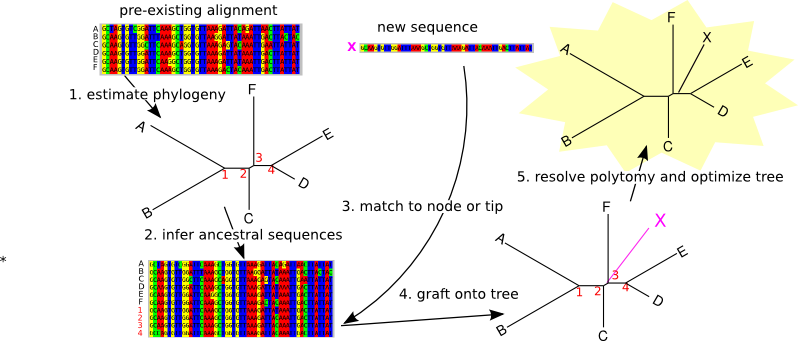
\includegraphics[scale=.7]{fig.png}
\end{center}
\caption{
{\bf Schematic of tree updating plan. \\
}  1) Estimate maximum likelihood phylogeny for starting set of taxa (A,B,C,D,E).
2) Create distributions of potential ancestral sequences at each node (numbered 1-4 here).
Only one potential reconstruction pictured.
3) Compare new taxon (X) to ancestral sequences.
4) Graft new taxon onto existing phylogeny, and add to alignment.
5) Update phylogeny under ML.
Working with the Stamatakis lab at HITS we will be able to optimize all of these steps and explore alternative options for tree updating.
}
\label{Figure_label}
\end{figure}

\subsection*{Maximum Likelihood Phylogenetics}
First we perform a full maximum likelihood estimation of the phylogeny for the alignment of the starting set of taxa, using RAxML \cite{stamatakis_RAxML_2014}, (Figure 1.1). 
While in the preliminary pipeline we move forward with only the maximum likelihood tree found in our search, we will test whether using a distribution of trees improves results. 
RAxML, developed by the Stamatakis lab the most computationally efficient approach to estimating maximum likelihood phylogenies available today. 
It has been optimized for use on high performance computing clusters \cite{stamatakis_raxml-vi-hpc:_2006} as well as for very large phylogenies\cite{stamatakis_RAxML-Light:_2012}.

\subsection*{Stochastic mapping of ancestral states}
From our starting tree we then generate a distribution of putative ancestral states for all nodes in the phylogeny, across all branches, using stochastic simulation of mutational histories. 
Stochastic simulation of mutations on phylogenies captures possible mutational histories along phylogenies \cite{nielsen_mapping_2002}\cite{huelsenbeck_stochastic_2003} and has been implemented both in a standalone GUI \cite{bollback_simmap:_2006} and as an R package \cite{revell_phytools:_2012}. 
Felsenstein's pruning algorithm \cite{felsenstein_evolutionary_1981}, upon which ML phylogenetic methods are based, calculates the probability of each base at each site at each node in the tree. 
The Stamatakis lab's Phylogenetic Likelihood Library (PLL) have a function to calculate these marginal ancestral sequences \url{http://www.libpll.org/}.
By using stochastic mapping we can derive a joint distribution of character states at each site across the tree, and combine those to form full joint distributions of putative alignments. 
Although generating these distributions is a computationally slow step, these alignments of putative ancestral states can be updated as new tips are added and do not need to be generated anew. 
Alternatively, Pupko\cite{pupko_fast_2000} \cite{Ashkenazy_FastML:_2012} has an algorithm for efficiently sampling the ML joint reconstruction at nodes. 
We can modify that algorithm to just sample from the posterior at nodes rather than along branches.
We will investigate the relative accuracy and efficiency of these different approaches.

\subsection*{Local alignments}
Following inference of ancestral states at nodes, we then take a new taxon sequenced for the same region, and perform BLAST\cite{altschul_gapped_1997} or Smith-Waterman\cite{rognes_faster_2011} searchers across each node within each stochastic iteration of ancestral state mappings. 
BLAST is an rapid search algorithm for DNA sequences that allows us to rapidly provisionally place new sequences at nodes in the tree. 
We will add the novel sequence to the multiple sequence alignment used to build the tree. 
We will compare alternative alignment techniques to determine the best approach to adding sequences, including profile based alignment \cite{loytynoja_accurate_2012} \cite{smith_mega-phylogeny_2009} and tracking insertion deletion histories using automata theory \cite{westesson_accurate_2012}.
PaPaRa \cite{Berger_aligning_2011} is a fast phylogeny informed method for accurately adding taxa to an alignment developed in the Stamatakis lab.


\subsection*{Re-optimization}
We then calculate the likelihood score for a new tree with this additional branch grafted on at the at location or locations suggested by the BLAST step. 
By using this new starting tree informed by ancestral state distributions, and building upon previous ML estimates of parameter values, we will be able to rapidly generate trees as good or better than those estimated from scratch. 

\subsection*{Testing}
We will thoroughly investigate several potential issues, including the impact of the addition order of taxa as we rebuild the tree, and whether global tree rearrangements are required on top of the process we propose.
We will compare the speed and accuracy of out taxon addition procedure to alternative taxon addition procedures as well as to full re-analyses.


\subsection*{Software}
When we have tested and determined an effective procedure for updating phylogenies with new sequences, we will develop an open source software package to be used by researchers in the field.

\subsection*{Advantages of collaboration with Stamatakis lab}

By collaborating with the Stamatakis lab I will be able to improve my skills in high performance computing and low level program optimization.
They have developed a parallelized software library, Phylogenetic Likelihood Library (PLL)  which we hope to leverage to speed up our calculations. 
In addition, I can work with the postdoc Dr. Tomas Flouri to incorporate the stochastic mapping of ancestral states into PLL.
By working directly with the Stamatakis lab I will be able to move forward without replicating work they have already accomplished.
I will be able to build upon their work on ExaBayes  \cite{Stamatakis_novel_2013} , EPA \cite{berger_performance_2011}, and PaPaRa  \cite{Berger_aligning_2011} .


\subsection*{Additional potential}
If development of tools for phylogeny updating is successful within the time frame of the project, there are many potential directions for expansion. 
While many phylogenies are currently built using information from a single gene, incorporating information from multiple loci makes inferences more robust \cite{edwards_looking_2009}. 
Rapid phlyogenetics at the single locus level can then be extended to genome scale analyses.
By speeding up updating of gene-trees, we can incorporate multiple gene trees into species phylogenies.
Ideally the software we develop for rapid phylogenetic updating can be incorporated into open online phylogeny resources, such as The Open Tree of Life project. 
This project, which Dr. 
Holder and myself are involved in, is building a synthetic phylogeny incorporating s many species as possible from across the tree of life. 
By integrating rapid phylogeny update tools with this online phylogeny repository we will be able to add taxa to this tree as data are processed, rather than the current lag time of moths or even years. 
Phylogenetic updating also has potential for rapid response to disease spread. 
Incorporating pathogen isolates into phylogenies can inform public health officials about the potential source \cite{timme_phylogenetic_2013}.
In addition, as genomic sequencing is becoming common across wide taxonomic breadth, imputed internal sequences can assist in homology searching.
Although PSI-BLAST \cite{altschul_gapped_1997} tries to exploit phylogenies, but using distributions of joint ancestral sequence samples could facilitate better detection of homology in distant comparisons.

         
\section*{Time schedule w/ milestones}
   Requested fellowship length: 9 months
 
\begin{itemize}
  \item{Months 1-2} Familiarize self with RAxML code and PLL library, with assistance of Stamatakis Lab. 
Develop C coding skills.
  \item{Month 3} Develop brute-force computational approaches and test if these methods are accurate using simulated data.
  \item{Month 4-6} Optimize and test code. Develop for distribution.
  \item{Months 7-8} Write manual and manuscript.
  \item{Month 9} Submission and revisions of manuscript.
\end{itemize}


\section*{Conclusions}
Much computational development will be necessary in order for evolutionary analysis to keep pace with the staggering rate of data generation. 
Although maximum likelihood methods estimating phylogenetic relationships are useful and are widely applied, new approaches are needed to build on large trees. 
The Stamatakis lab has been at the forefront of development of efficient tools for phylogenetic analysis, and by working with them I will be able to build upon their expertise. 
We propose to develop a better approach for adding new taxa onto existing phylogenies that combines the advantages of using complex models of sequences evolution and maximum likelihood analysis with the speed needed to keep up with the stream of new biological sequence data. 

\pagebreak

\bibliography{Humboldt}



\end{document}

